\documentclass[a4paper,norsk]{article}
\usepackage{preamble}
\usepackage{tabu}
\usepackage{color, colortbl}
\definecolor{LightCyan}{rgb}{0.88,1,1}

\begin{document}

\section*{TASK 2: Discretization of convection/diffusion}
\textbf{Derive a proper variational formulation of the convection/diffusion 
problem.  Derive sucient conditions that make the problem well-posed.  Discuss
why oscillations appear for standard Galerkin methods and show how SUPG
methods resolve these problems.  Discuss also approximation properties in
light of Cea's lemma.}\newline \newline

The convection–diffusion equation is a combination of the diffusion and convection (advection) equations, and describes physical phenomena where particles, energy, or other physical quantities are transferred inside a physical system due to two processes
\begin{align*}
\mu \nabla^2 u +v \cdot \nabla u = f \hspace{1mm} \in \Omega \\
u = g \hspace{1mm} \in \partial \Omega
\end{align*}

\begin{itemize}
\item u = Is the 
\item $\mu \nabla^2 u$ = Diffusion term, distribution of consentration due to consentration differene (Ink in glass..)
\item $\mu$ = Dynamic viscoucity
\item $v \cdot \nabla u $ = Convection(Advection), distribution of consentration due to fluid flow
\item v = Can bee fluid flow average, etc..
\end{itemize}

\subsection*{Singular Pertubation problem}
Consequence $\mu \rightarrow 0$, boundary conditions can't be satisfied. Changes the very nature of problem.
Practical situations $\mu > 0$, but small in the sence that $\mu << |v|$. This results in a overdetermined problem. (Also if $\mu$ goes to 0).
For such problem where $\mu << |v|$, solution will be similar to  $\mu = 0$, EXCEPT close to \textbf{NON-inflow boundary}. Here we will typically have a boundary layer.
We will also observe that the discretized problem, will result in unphysical oscillations starting at this boundary layer.

\newpage
\subsection{1D con-diff problem}
\begin{align*}
\ u_x - \mu u_{xx}  = 0 \\
u(0) = 0 \hspace{2mm} u(1) = 1 \\
u_e(x) = \frac{e^{\frac{-x}{\mu}} -1}{e^{\frac{-1}{\mu}} - 1}
\end{align*}

For $\mu \rightarrow 0$ both $e^{\frac{-x}{\mu}}$ and $e^{\frac{-1}{\mu}}$ and $u(x) \approx 1$ unless $x \approx 0$. Close to the inflow boundary
x = 0, there will be a boundary layer where u has exponential growth.
\newline \textbf{Galerkin method} \newline

Find $u \in  H^1_{0,1}$ such that 
\begin{align*}
\int_0^1 \big( u_x v - \mu u_{xx} v \big) \hspace{1mm} dx = 0 \\
\inner[-u_x]{v} \hspace{2mm} \mu \inner[\nabla u]{\nabla v} = 0 \hspace{2mm}  \forall v \in H^1_{0,0}
\end{align*}

\begin{figure}[h!]
	\centering
	\caption*{CONVEC N = 20 and N = 100}
	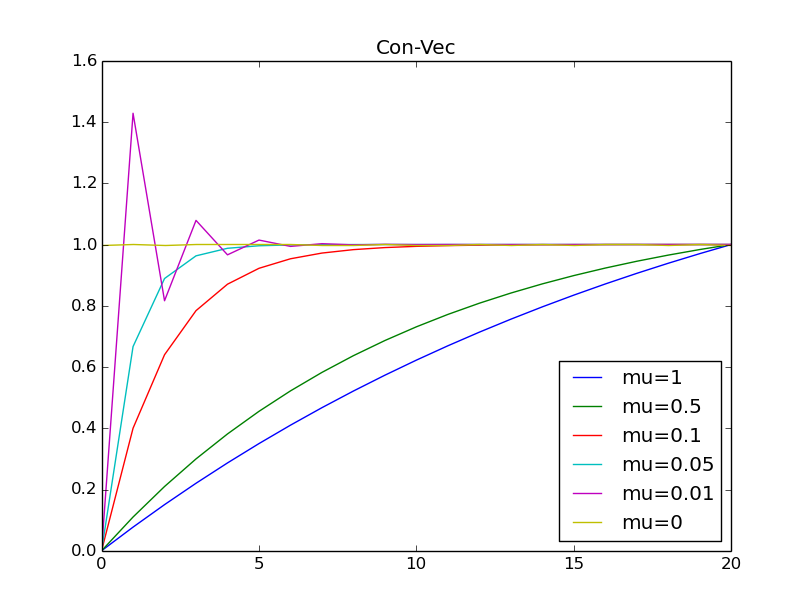
\includegraphics[scale=0.36]{convec.png}
	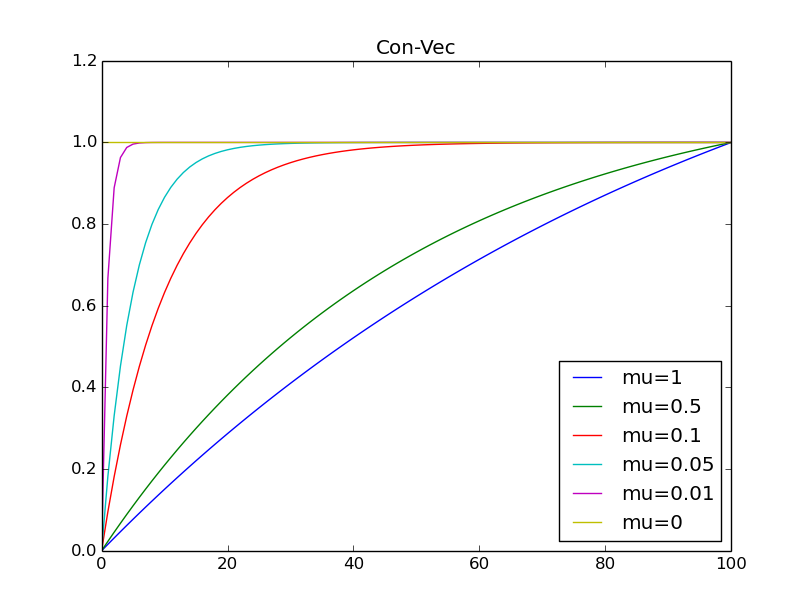
\includegraphics[scale=0.36]{convechighn.png}
\end{figure}
Observe oscillations for low choice of N. WHY DO THIS HAPPEND? Explain with FDM.
\newpage
Using central difference
\begin{align*}
&\frac{\mu}{h^2}\Big[u_{i+1} - 2u_{i} + u_{i-1} \Big] - \frac{v}{2 h} \Big[u_{i+1} - u_{i-1} \Big] = 0 \\
&u_0 = 0 \hspace{2mm} u_N = 1 \hspace{3mm} \\ 
\text{for} \hspace{2mm} \mu = 0 \\
&\frac{v}{2 h} \Big[u_{i+1} - u_{i-1} \Big] = 0 \hspace{3mm} u_{i+1} = u_{i-1} \hspace{2mm} \textbf{SOURCE OSCILLATIONS}
\end{align*}
\textbf{THE CURE} Introduce and artifical diffusion term. \\ drop central difference scheme, use upwind such that 
\begin{align*}
\pd[u]{x} (x_i) = \frac{u_{i+1}-u_{i}}{h} \hspace{2mm} v < 0 \\
\pd[u]{x} = \frac{u_{i}-u_{i-1}}{h} \hspace{2mm} v > 0
\end{align*}
\begin{itemize}
\item \textbf{PROS} = Oscillations dissapear
\item \textbf{CONS} = 1 order convergence
\end{itemize}
\textbf{POINT!} Show relation to \textbf{upwind} and \textbf{artifical diffusion}
Observe 
\begin{align*}
\frac{u_{i+1}-u_{i-1}}{2h} \hspace{2mm} \text{Central Scheme, 1. order convergence} \\
\end{align*}
 




\end{document}
